\documentclass[11pt,a4paper]{article}
\usepackage{tikz}
\usetikzlibrary{arrows.meta,positioning}
\usepackage{tabularx}
\usepackage{amsmath,amssymb,amsthm}
\usepackage{geometry}
\geometry{margin=1in}
\usepackage{hyperref}
\usepackage{graphicx}
\usepackage{setspace}
\onehalfspacing

\title{\textbf{Paper F-04: Nuclear Dynamics:\\ A Constraint-Driven Flux Dynamics (CDFD) Perspective}}
\author{Steve Bico Mujjabi, MD\\
\small Independent Researcher\\
\small Founder, Vura Labs\\
\small Kampala, Uganda\\
\small ORCID: 0009-0001-0556-5516}
\date{August 2026}

\begin{document}
\maketitle

% BEGIN SHARED-METHODS POINTER
\noindent\textit{Shared Part IV notation and evidence boundaries are defined in \path{PART_IV_METHODS_AND_CLAIM_BOUNDARY.md}. This paper states only its local observables, comparison, and failure conditions.}
% END SHARED-METHODS POINTER


\begin{abstract}
This paper develops a falsifiable CDFD/AFL model of Nuclear Dynamics. It maps particle, energy, and reaction fluxes to driving flux $\Phi$, binding, conservation laws, Coulomb barriers, and available states to active constraint $C$, decay, reaction channels, collective modes, and energy redistribution to responsiveness $S$, and isotopic composition, excitation, deformation, and reaction history to structural memory $M_s$. The target outcome is stability, yields, decay pathways, and energy release, tested against cross sections, decay data, spectroscopy, collision experiments, and nuclear models. The paper treats universality as a shared model architecture rather than an assertion that unlike systems have the same material mechanism. It states the negative result that would make the mapping unnecessary and places the domain claim inside the cumulative CDFD programme and its reproducible runtime boundary.
\end{abstract}

\section{Introduction}

At the femtometer scale, the atomic nucleus is a highly dense, dynamic droplet of nucleons bound together by the residual strong force. The balance of forces within the nucleus dictates the stability of all matter in the universe. While quantum chromodynamics (QCD) describes the fundamental quark-gluon interactions, describing bulk nuclear phenomena (such as fission and alpha decay) requires a macro-scale thermodynamic approach.

CDFD offers a unified thermodynamic ontology. Whether analyzing a living biological cell or an atomic nucleus, the system must maintain sufficient internal throughput to offset its structural constraints. In the nucleus, this throughput is the continuous exchange of virtual mesons (primarily pions) between nucleons.

\section{The Nuclear Adaptive Surface}
We model the atomic nucleus as an active surface characterized by the CDFD scaling equation:
\begin{equation}
    \Psi_s = \left( \frac{\Phi}{C} \right) \cdot S \cdot M_s
\end{equation}

For a nucleus composed of $Z$ protons and $N$ neutrons, the parameters map as follows:
\begin{itemize}
    \item \textbf{Flux ($\Phi$)}: The strong force mediated nucleon-nucleon exchange. This flux scales with the total number of adjacent nucleon pairs, roughly proportional to the nuclear volume $A = Z+N$.
    \item \textbf{Constraint ($C$)}: The disruptive Coulomb repulsion between protons, which scales as $Z^2 / A^{1/3}$, along with the Pauli exclusion principle which forces nucleons into higher energy states.
    \item \textbf{Responsiveness ($S$)}: The binding energy per nucleon, indicating the depth of the local potential well and the surface tension of the nuclear droplet.
    \item \textbf{Memory ($M_s$)}: Nuclear shell structure. Nuclei with "magic numbers" of protons or neutrons exhibit closed shells, locking the nuclear topology into a highly efficient, rigid state (perfect memory, $M_s \to 1.0$).
\end{itemize}

\subsection{Nuclear Decay as Adaptive Failure}
A stable nucleus maintains $\Psi_s \approx 1$. The cohesive flux of the strong force perfectly regulates the outward pressure of the Coulomb constraint.

As we move to heavy elements (increasing $Z$), the Coulomb constraint $C \propto Z^2$ grows much faster than the strong force flux $\Phi \propto A$. Consequently, the ratio $(\Phi/C)$ begins to plummet. To prevent the system from entering a catastrophic decay regime ($\Psi_s \ll 1$), the nucleus must adapt by increasing its neutron-to-proton ratio, effectively boosting $\Phi$ without adding to $C$.

However, eventually, the surface responsiveness $S$ reaches a saturation limit. The nucleus can no longer bind the excess neutrons effectively due to the Pauli constraint. The system memory $M_s$ locks into a state of chronic overload. The nucleus violently sheds the excess constraint through Alpha decay or spontaneous fission, fracturing the system to restore $\Psi_s \approx 1$ in the resulting daughter nuclei.



\section{Measurement Layer}

% BEGIN PART IV MAJOR CROSS-DOMAIN UPGRADE
\section{Cross-Domain Model Upgrade: Mechanism, Scale, and Tests}

\subsection{Observable Translation}

The paper-specific translation begins with an observable chain rather than a
verbal analogy. For Nuclear Dynamics, the proposed drive is particle, energy, and reaction fluxes.
The active limitation is binding, conservation laws, Coulomb barriers, and available states. Responsiveness is carried by
decay, reaction channels, collective modes, and energy redistribution, while retained state is represented by
isotopic composition, excitation, deformation, and reaction history. The outcome to explain is stability, yields, decay pathways, and energy release.

\begin{table}[htbp]
\centering
\small
\caption{Operational CDFD/AFL map for Paper F-04.}
\begin{tabularx}{\textwidth}{|l|X|X|}
\hline
\textbf{Term} & \textbf{Paper-specific observable meaning} & \textbf{Measurement question} \\
\hline
$\Phi$ & particle, energy, and reaction fluxes & What rate, load, gradient, or demand enters the focal system? \\
\hline
$C$ & binding, conservation laws, Coulomb barriers, and available states & Which measured bottleneck limits transfer, function, or recovery? \\
\hline
$S$ & decay, reaction channels, collective modes, and energy redistribution & Which process changes effective capacity or reroutes the load? \\
\hline
$M_s$ & isotopic composition, excitation, deformation, and reaction history & Which retained state makes equal present loads produce different futures? \\
\hline
$Y$ & stability, yields, decay pathways, and energy release & Which outcome is predicted out of sample, with uncertainty? \\
\hline
\end{tabularx}
\end{table}

\begin{figure}[htbp]
\centering
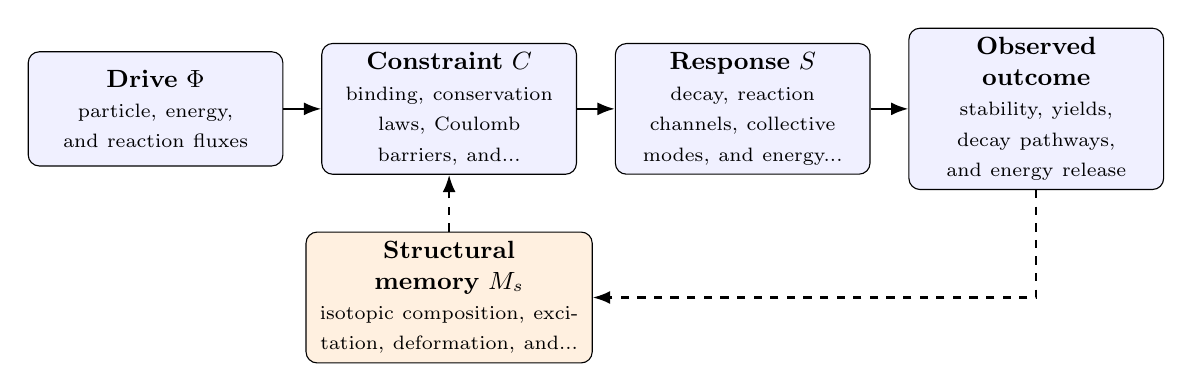
\begin{tikzpicture}[
    node distance=0.48cm,
    every node/.style={font=\small},
    box/.style={draw, rounded corners, align=center, minimum height=1.45cm, text width=3.0cm, fill=blue!6},
    memory/.style={draw, rounded corners, align=center, minimum height=1.25cm, text width=3.4cm, fill=orange!12},
    flow/.style={-{Latex[length=2.2mm]}, thick},
    feedback/.style={-{Latex[length=2.2mm]}, thick, dashed}
]
\node[box] (drive) {\textbf{Drive $\Phi$}\\\scriptsize particle, energy, and reaction fluxes};
\node[box, right=of drive] (constraint) {\textbf{Constraint $C$}\\\scriptsize binding, conservation laws, Coulomb barriers, and...};
\node[box, right=of constraint] (response) {\textbf{Response $S$}\\\scriptsize decay, reaction channels, collective modes, and energy...};
\node[box, right=of response] (outcome) {\textbf{Observed outcome}\\\scriptsize stability, yields, decay pathways, and energy release};
\node[memory, below=0.72cm of constraint] (memory) {\textbf{Structural memory $M_s$}\\\scriptsize isotopic composition, excitation, deformation, and...};
\draw[flow] (drive) -- (constraint);
\draw[flow] (constraint) -- (response);
\draw[flow] (response) -- (outcome);
\draw[feedback] (outcome.south) |- (memory.east);
\draw[feedback] (memory.north) -- (constraint.south);
\end{tikzpicture}
\caption{Paper F-04 observable CDFD/AFL architecture for Nuclear Dynamics. Solid arrows give the proposed forward chain; dashed arrows make history-dependent feedback explicit.}
\label{fig:f04-architecture}
\end{figure}

\subsection{Paper-Specific Causal Hypothesis}

For this paper, the hypothesized causal sequence is specific. A change in
particle, energy, and reaction fluxes arrives faster than decay, reaction channels, collective modes, and energy redistribution can compensate.
This raises or redistributes binding, conservation laws, Coulomb barriers, and available states. If the load persists,
the retained state encoded by isotopic composition, excitation, deformation, and reaction history changes the next response, so a later event of equal
magnitude can produce a different trajectory in stability, yields, decay pathways, and energy release. The
scientific task is to estimate that sequence against the best ordinary model of
the domain, not merely to redescribe the outcome after it occurs.

\subsection{Cross-Scale Translation Without Mechanistic Erasure}

For the cosmic and subatomic systems family, the cross-domain translation must remain subordinate to conservation laws, relativity, quantum mechanics, and established astrophysical or plasma equations. CDFD is useful only if it compresses a regime transition or hysteresis question without pretending that biological adaptation and physical response are the same mechanism. \cite{Turing1952,Shannon1948,BakTangWiesenfeld1987}
The required scale declaration for this paper is attoseconds to geological time; nucleons to astrophysical reaction networks. At short
scales, the key question is whether the incoming drive is transmitted,
buffered, or diverted. At intermediate scales, response changes effective
capacity and network exposure. At long scales, retained structure can alter the
state space itself. A result is genuinely cross-scale only when the aggregation
rule is stated and the same conclusion is not an artifact of averaging.

\subsection{Evidence Ladder and Discriminating Tests}

\begin{table}[htbp]
\centering
\small
\caption{Evidence ladder for Paper F-04. Each rung can fail independently.}
\begin{tabularx}{\textwidth}{|p{0.17\textwidth}|X|X|}
\hline
\textbf{Test} & \textbf{Design} & \textbf{Discriminating result} \\
\hline
Proxy audit & Measure cross sections, decay data, spectroscopy, collision experiments, and nuclear models and preregister how each record maps to $\Phi$, $C$, $S$, $M_s$, and $Y$. & The mapping fails if proxies are non-identifiable, circular, or change meaning across cases. \\
\hline
Load ramp & Apply or observe a controlled energy or particle-flux scan across isotopes while estimating the dominant constraint and response time. & A threshold claim requires a reproducible nonlinear change and uncertainty bounds, not a visually chosen breakpoint. \\
\hline
Recovery and memory & Match present load across units with different histories, then compare recovery paths. & The memory claim requires history-dependent divergence after current conditions are controlled. \\
\hline
Model comparison & Compare the baseline domain model with and without the CDFD/AFL state variables using held-out data. & The paper's stated falsifier is: the translation adds no testable structure beyond established nuclear theory. \\
\hline
\end{tabularx}
\end{table}

\subsection{Research Programme and Boundary Conditions}

The immediate research programme has four steps. First, construct a documented
dataset from cross sections, decay data, spectroscopy, collision experiments, and nuclear models and retain raw units before normalization.
Second, fit a baseline domain model and report its calibration and out-of-sample
error. Third, add the smallest identifiable CDFD/AFL state extension and test
whether it improves prediction of stability, yields, decay pathways, and energy release. Fourth, repeat the
analysis across the declared scale range and publish negative cases as part of
the cross-domain translation audit.

% END PART IV MAJOR CROSS-DOMAIN UPGRADE

\section{Conclusion}
Radioactive decay is not a random violation of stasis; it is the necessary, model-predicted response of an active system failing to maintain adequate throughput against rising constraints. By framing nuclear dynamics as an Adaptive Flux Limited system, we bridge the gap between subatomic quantum mechanics and universal macroscopic thermodynamics, revealing that the atomic nucleus breathes and regulates its structural topology exactly like an organic cell.
\section*{Conflict of Interest} The author declares no conflict of interest.
\section*{Data Availability}
Part-specific runtime diagnostics are under each Part's \path{outputs/} directory.

Release-wide code: \path{Part_E_Synthesis/supplementary/}.

Generated summaries: \path{Part_E_Synthesis/outputs/}.

Figures: \path{Part_E_Synthesis/figures/}.


\section{Reference Layer}
\bibliographystyle{plain}
\bibliography{universal_afl_references}
\end{document}
